\section{Integration Strategy}

\subsection{Entry Criteria}
Before integration tests may begin all the primary functions and components of the application must be finished and working.
Specifically: registration, login, requests, reservation and taxi sharing functions must work as planned. To do so all the components listed in the design document must be working as well. Exception made for the user interface component.

\subsection{Elements to be Integrated}
The components to be integrated are:
\begin{itemize}
	\item Client component
	\item Ride manager component
	\item User manager component. 
\end{itemize}
For a more detailed description on how these components should work refer to architectural design section of the Design Document

\subsection{Integration Testing Strategy}
We will adopt a bottom-up testing strategy, integrating first the sub-components and later on the higher level. 
We choose this strategy because the sub-components of our system are independent one to each other and they can be integrated separately.

\subsection{Sequence of Component}
Since we adopt a bottom-up integration strategy, we will start from the lower level component (database), then the components that directly access the database, thus account and rider creator, then the manager of those components and finally the user interface.
\begin{figure}[h]
		\centering
		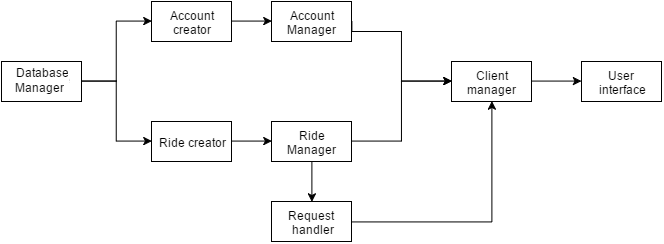
\includegraphics{subsystem.png}
		\caption{This flowchart show the sequence of integration of the components}
\end{figure}
